\begin{figure}[h!]
	\centering
	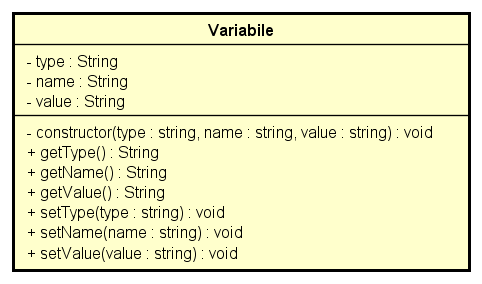
\includegraphics[scale=0.8]{res/sections/SpecificaFrontEnd/Services/Disegnetti/variabile.png}
	\caption{Diagramma della classe Variabile}
\end{figure}

\begin{itemize}
	\item \textbf{Descrizione:}\\
	
	\item \textbf{Utilizzo:}\\
	
	\item \textbf{Metodi:}
		\begin{itemize}
			\item \emph{-type: string}\\
    		
    		\item \emph{-name: string}\\
    		
    		\item \emph{-value: string}\\
    		
		\end{itemize}
	\item \textbf{Metodi:}
		\begin{itemize}
			\item \emph{-constructor(type: string, name: string, value: string)}\\
    		\\
    		\textbf{Parametri:}
    		\begin{itemize}
    			\item \emph{type: string}\\
    			
    			\item \emph{name: string}\\
    			
    			\item \emph{value: string}\\
    			
    		\end{itemize}
    		\item \emph{+getType()}\\
    		
    		\item \emph{+getName()}\\
    		
    		\item \emph{+getValue()}\\
    		
    		\item \emph{+setType(type: string)}\\
    		\\
    		\textbf{Parametri:}
    		\begin{itemize}
    			\item \emph{type: string}\\
    			
    		\end{itemize}
    		\item \emph{+setName(name: string)}\\
    		\\
    		\textbf{Parametri:}
    		\begin{itemize}
    			\item \emph{name: string}\\
    			
    		\end{itemize}
    		\item \emph{+setValue(value: string)}\\
    		\\
    		\textbf{Parametri:}
    		\begin{itemize}
    			\item \emph{value: string}\\
    			
    		\end{itemize}
    	\end{itemize}
\end{itemize}